\documentclass{article}
\usepackage{booktabs} 
\usepackage{geometry}
\usepackage{longtable}
\usepackage[dvipsnames,table]{xcolor}
\usepackage{fancyhdr}
\usepackage{xcolor}
\usepackage{graphicx}
\usepackage{hyperref}
\usepackage{float}
\usepackage{listings}
\usepackage{amssymb}
\usepackage{amsmath}
\usepackage{enumitem}
\usepackage{parskip}
\usepackage{listing}
\usepackage[table]{xcolor}
\usepackage{longtable}
\usepackage{colortbl}
\usepackage[dvipsnames,table]{xcolor}
\usepackage{caption}       % For \captionof
\usepackage{tabularx}      % For tables with adjustable-width columns
\usepackage{circuitikz}    % For circuit diagrams

% Choose paper size
\geometry{letterpaper, top=25.4mm, bottom=25.4mm, left=25.4mm, right=25.4mm}

\color{black}
\fancyhf{}
\renewcommand{\headrulewidth}{1pt}
\renewcommand{\footrulewidth}{1pt}

% Define standard IPF color palette
\definecolor{soft-sky-blue}{HTML}{B7DAEB}
\definecolor{orange}{HTML}{FF6633}
\definecolor{cool-grey}{HTML}{91A1B0}
\definecolor{black}{HTML}{000000}
\definecolor{space-blue}{HTML}{003366}
\definecolor{pigeon-blue}{HTML}{5F8396}
\definecolor{sage-green}{HTML}{95A077}
\definecolor{fire-yellow}{HTML}{F9A651}
\definecolor{apple-red}{HTML}{CC4200}
\definecolor{crockadile-green}{HTML}{718944}
\definecolor{slate-grey}{HTML}{607587}
\definecolor{fog-grey}{HTML}{E5E6E9}

% Define certification colors
\definecolor{cert-level-0}{HTML}{CC4200} % apple-red
\definecolor{cert-level-1}{HTML}{FF6633} % orange
\definecolor{cert-level-2}{HTML}{F9A651} % fire-yellow
\definecolor{cert-level-3}{HTML}{B7DAEB} % soft-sky-blue
\definecolor{cert-level-4}{HTML}{5F8396} % pigeon-blue
\definecolor{cert-level-5}{HTML}{718944} % sage-green

\hypersetup{hidelinks}
\pagestyle{fancy}
\pagenumbering{arabic}

\title{

\includegraphics[width=8cm] {images/Rocksavage_Tech_RGB_300.png}\vspace{50pt}
\vspace{10pt} \\
\textbf{UART \\
  Product User Guide} \\
{\small{\textcolor{slate-grey}{rocksavagetech.chiselWare.UART}}} \\
\vspace{20pt} IPF certified to level:
\textbf{\textcolor{cert-level-0}{0} }of 5 \\
\vspace{5pt}

\includegraphics[width=4cm] {images/uncertified.png}
}

\author{Warren Savage}

\fancyhead[L]{UART Users Guide}
\fancyhead[R]{\leftmark}
\fancyfoot[C]{Rocksavage Technology, Inc.~\copyright~2023}
\fancyfoot[R]{Page \thepage}

\begin{document}

\maketitle
\newpage
\tableofcontents

% -- Include subfiles, in parallel to how your I2C doc is structured
\section{Errata and Known Issues}

\subsection{Errata}
\begin{itemize}
    \item It should be noted that the baud rate is set by an interative divider. It can take up to 32 clock cycles to converge to a division result.
\end{itemize}

\subsection{Known Issues}
None.
\section{Port Descriptions}

The UART module provides two sets of ports:
\begin{enumerate}
  \item The external UART interface (serial TX and RX signals)
  \item The APB interface for register access
\end{enumerate}

\subsection{UART Interface}

The UART-specific ports allow the module to communicate with external devices over a standard asynchronous serial link. The key signals are:

\renewcommand*{\arraystretch}{1.3}
\begingroup
\small
\rowcolors{2}{gray!30}{gray!10}
\begin{longtable}[H]{
  | p{0.25\textwidth}
  | p{0.15\textwidth}
  | p{0.15\textwidth}
  | p{0.40\textwidth} |
}
\hline
\rowcolor{gray}
\textcolor{white}{\textbf{Port Name}} &
\textcolor{white}{\textbf{Width}} &
\textcolor{white}{\textbf{Direction}} &
\textcolor{white}{\textbf{Description}} \\ \hline
\endfirsthead

\hline
\rowcolor{gray}
\textcolor{white}{\textbf{Port Name}} &
\textcolor{white}{\textbf{Width}} &
\textcolor{white}{\textbf{Direction}} &
\textcolor{white}{\textbf{Description}} \\ \hline
\endhead

\hline
\endfoot

\texttt{rx} &
1 &
Input &
Asynchronous serial receive data input. This signal is synchronized internally and sampled by the receiver FSM. \\ \hline

\texttt{tx} &
1 &
Output &
Serial transmit data output. When idle, this line remains high. \\ \hline
\end{longtable}
\captionof{table}{UART Interface Ports}
\label{table:uart_ports}
\endgroup

\subsection{APB Interface}

The APB interface provides access to the UART’s registers, allowing software to configure and monitor both the TX and RX operations (including baud rate settings, FIFO control, and error status). The APB signals are defined as follows:

\renewcommand*{\arraystretch}{1.3}
\begingroup
\small
\rowcolors{2}{gray!30}{gray!10}
\begin{longtable}[H]{
  | p{0.20\textwidth}
  | p{0.20\textwidth}
  | p{0.12\textwidth}
  | p{0.43\textwidth} |
}
\hline
\rowcolor{gray}
\textcolor{white}{\textbf{Port Name}} &
\textcolor{white}{\textbf{Width}} &
\textcolor{white}{\textbf{Direction}} &
\textcolor{white}{\textbf{Description}} \\ \hline
\endfirsthead

\hline
\rowcolor{gray}
\textcolor{white}{\textbf{Port Name}} &
\textcolor{white}{\textbf{Width}} &
\textcolor{white}{\textbf{Direction}} &
\textcolor{white}{\textbf{Description}}\\ \hline
\endhead

\hline
\endfoot

\texttt{PCLK} &
1 &
Input &
APB clock signal for register access. \\ \hline

\texttt{PRESETN} &
1 &
Input &
Active–low asynchronous reset. \\ \hline

\texttt{PSEL} &
1 &
Input &
Select signal indicating that the UART is addressed. \\ \hline

\texttt{PENABLE} &
1 &
Input &
Indicates the second cycle of an APB transfer. \\ \hline

\texttt{PWRITE} &
1 &
Input &
Determines the operation: HIGH for write, LOW for read. \\ \hline

\texttt{PADDR} &
\textit{addressWidth} &
Input &
APB address bus for register selection. \\ \hline

\texttt{PWDATA} &
\textit{dataWidth} &
Input &
APB write data bus. \\ \hline

\texttt{PRDATA} &
\textit{dataWidth} &
Output &
APB read data bus. \\ \hline

\texttt{PREADY} &
1 &
Output &
Indicates that the UART is ready for the next transfer. \\ \hline

\texttt{PSLVERR} &
1 &
Output &
Indicates a transfer error. \\ \hline
\end{longtable}
\captionof{table}{APB Interface Ports}
\label{table:apb_ports}
\endgroup

\section{Parameter Descriptions}

Table~\ref{table:params} summarizes the key parameters for the \textbf{UART} module. Each can be customized during instantiation.

\renewcommand*{\arraystretch}{1.3}
\begingroup
\small
\rowcolors{2}{gray!30}{gray!10}
\arrayrulecolor{gray!80}

\begin{longtable}[H]{
  | p{0.22\textwidth}
  | p{0.13\textwidth}
  | p{0.08\textwidth}
  | p{0.08\textwidth}
  | p{0.42\textwidth} |
}
\hline
\rowcolor{gray}
\textcolor{white}{\textbf{Name}} &
\textcolor{white}{\textbf{Type}} &
\textcolor{white}{\textbf{Min}} &
\textcolor{white}{\textbf{Max}} &
\textcolor{white}{\textbf{Description}} \\ 
\hline
\endfirsthead

\hline
\rowcolor{gray}
\textcolor{white}{\textbf{Name}} &
\textcolor{white}{\textbf{Type}} &
\textcolor{white}{\textbf{Min}} &
\textcolor{white}{\textbf{Max}} &
\textcolor{white}{\textbf{Description}} \\ 
\hline
\endhead

\hline
\endfoot

\texttt{dataWidth} &
Integer &
8 &
32 &
Data width for APB bus operations. \\ \hline

\texttt{addressWidth} &
Integer &
1 &
-- &
Address width for APB bus. \\ \hline

\texttt{maxClocksPerBit} &
Integer &
2 &
-- &
Maximum allowed clock cycles per UART bit. Determines maximum baud rate. \\ \hline

\texttt{maxOutputBits} &
Integer &
5 &
16 &
Maximum number of data bits plus optional parity bit. Typically up to 9 or so, here parameterized. \\ \hline

\texttt{fifoDepth} &
Integer &
1 &
-- &
Depth of the internal RX/TX FIFOs. Must be a power of 2. \\ \hline

\texttt{syncDepth} &
Integer &
2 &
-- &
Depth for RX input synchronization. Recommended at least 2 for metastability protection. \\ \hline

\texttt{parity} &
Bool &
N/A &
N/A &
Default parity selection (odd/even). This can be overridden by registers at runtime. \\ \hline

\texttt{verbose} &
Bool &
N/A &
N/A &
Enables debugging \texttt{printf} statements. \\ \hline

\end{longtable}
\captionof{table}{UART Parameter Descriptions}
\label{table:params}
\endgroup

\noindent
A typical instantiation in Scala might look like:
\begin{lstlisting}[language=Scala]
// Example instantiation
val myUart = Module(new Uart(
  UartParams(
    dataWidth       = 32,
    addressWidth    = 32,
    maxClocksPerBit = 217,
    maxOutputBits   = 8,
    fifoDepth       = 16,
    syncDepth       = 2,
    parity          = false,
    verbose         = false
  ),
  formal = false
))
\end{lstlisting}

\section{Operating Modes}

The UART module is designed for full–duplex asynchronous serial communication.
It implements independent transmitter (TX) and receiver (RX) paths that operate concurrently.
Both paths include configurable settings for baud rate, data length, and parity.
In addition, each side incorporates an internal FIFO buffer to decouple external data handling
from the serial transmission or reception.

\begin{figure}[H]
    \centering
    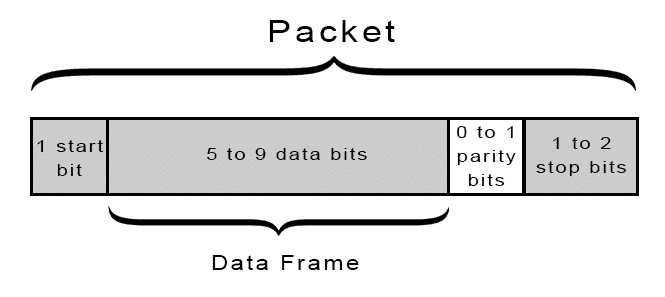
\includegraphics[width=0.85\textwidth]{images/frame_format.png}
    \caption{Frame Formats}
    \label{fig:frame_formats}
  \end{figure}

\subsection{Modes}

\begin{itemize}
    \item \textbf{Data Buffering:} 
    \begin{itemize}
        \item Software writes data into the \texttt{TX\_DATA\_IN} register which automatically write into the FIFO.
        \item A send trigger (e.g., pulsing \texttt{TX\_LOAD}) pops all data from the FIFO in the order it came in one after the other.
    \end{itemize}
    
    \item \textbf{Baud Rate Updating:}
    \begin{itemize}
        \item The Both the TX and RX paths include dedicated \texttt{UartBaudRateGenerator} modules.
        \item Software sets the desired baud rate and clock frequency via registers (\texttt{TX\_BAUD\_RATE} and \texttt{TX\_CLOCK\_FREQ}) and then pulses the update control (e.g., \texttt{TX\_UPDATE\_BAUD}).
        \item The transmitter enters a \texttt{BaudUpdating} state. The baud generator computes the effective \texttt{clocksPerBit} (i.e. the number of system clocks per transmitted bit) and asserts a \texttt{baudValid} signal when complete.
        \item Once valid, the computed divisor is stored in \texttt{clocksPerBitReg} and the state machine transitions back to \texttt{Idle}.
    \end{itemize}
    
    \item \textbf{Data Transmission:}
    \begin{itemize}
        \item Upon detecting that data is available in the FIFO and the transmitter is idle, the state machine initiates a new transmission by loading the next word from the FIFO.
        \item Before transmission begins, the TX data word is “reversed” (using an internal \texttt{reverse()} function) so that the least-significant bit (LSB) is transmitted first.
        \item The transmission sequence then follows standard UART timing:
            \begin{enumerate}[noitemsep]
                \item \textbf{Start Bit:} A start bit (\texttt{0}) is driven.
                \item \textbf{Data Bits:} The state machine shifts out the configured number (\texttt{TX\_NUM\_OUTPUT\_BITS\_DB}) of data bits in the \texttt{Data} state.
                \item \textbf{Parity Bit (Optional):} If parity is enabled (\texttt{TX\_USE\_PARITY\_DB}=1), a parity bit is computed from the full (unshifted) data word and transmitted in the \texttt{Parity} state. The selection of odd or even parity is controlled by \texttt{TX\_PARITY\_ODD\_DB}.
                \item \textbf{Stop Bit:} Finally, one or more stop bits (\texttt{1}) are transmitted in the \texttt{Stop} state.
            \end{enumerate}
        \item During transmission, the TX output (\texttt{tx}) is driven accordingly. When idle, \texttt{tx} remains high.
    \end{itemize}
    
    \item \textbf{State Machine Overview:}
    \begin{itemize}
        \item The TX state machine transitions through the following key states:
            \begin{itemize}
                \item \texttt{Idle}: Waiting for new data and/or baud update.
                \item \texttt{BaudUpdating}: Waiting for the baud rate generator to compute \texttt{clocksPerBit}.
                \item \texttt{Start}: Driving the start bit.
                \item \texttt{Data}: Shifting out the data bits.
                \item \texttt{Parity}: (Optional) Transmitting the parity bit.
                \item \texttt{Stop}: Driving the stop bit(s) before returning to \texttt{Idle}.
            \end{itemize}
        \item The signal \texttt{startTransaction} is generated when a new word is ready (from FIFO) and the transmitter is idle.
        \item The computed \texttt{clocksPerBit} governs the timing of data sampling and shifting.
    \end{itemize}
\end{itemize}

\subsection{Receiver Mode}

In receiver mode, the UART receiver continuously monitors the \texttt{rx} input and performs the following functions:

\begin{itemize}
    \item \textbf{Signal Synchronization:}
    \begin{itemize}
        \item The asynchronous \texttt{rx} input is first passed through a chain of flip–flops (of depth defined by \texttt{syncDepth}) to mitigate metastability.
        \item The synchronized signal (\texttt{rxSync}) is used for all subsequent sampling.
    \end{itemize}
    
    \item \textbf{Baud Rate Updating:}
    \begin{itemize}
        \item Similar to the transmitter, the RX path uses a \texttt{UartBaudRateGenerator}.
        \item Software sets the RX baud rate and clock frequency using registers (e.g., \texttt{RX\_BAUD\_RATE} and \texttt{RX\_CLOCK\_FREQ}) and then pulses \texttt{RX\_UPDATE\_BAUD}.
        \item The RX state machine enters a \texttt{BaudUpdating} state, during which the effective \texttt{clocksPerBit} is calculated and stored in \texttt{clocksPerBitReg}.
        \item Once the baud generator asserts \texttt{baudValid}, the FSM transitions back to \texttt{Idle} and resumes monitoring.
    \end{itemize}
    
    \item \textbf{Data Reception:}
    \begin{itemize}
        \item The receiver continuously samples the \texttt{rxSync} signal.
        \item A falling edge (transition from high to low) indicates a start bit, and the receiver then enters the \texttt{Start} state.
        \item After a fixed delay (approximately half the duration of a bit period), the receiver begins to sample the incoming data bits in the \texttt{Data} state.
        \item If parity is enabled (\texttt{RX\_USE\_PARITY\_DB}=1), the FSM transitions to the \texttt{Parity} state and compares the received parity bit against the expected value. The expected parity is computed from the shifted–in data and the setting of \texttt{RX\_PARITY\_ODD\_DB}.
        \item Finally, the receiver checks the stop bit in the \texttt{Stop} state. If the stop bit is not detected (i.e., if the line is not high at the end of the bit period), a framing error is flagged.
    \end{itemize}
    
    \item \textbf{Data Buffering:}
    \begin{itemize}
        \item Once a complete frame is successfully received (with no errors), the RX data is latched and then pushed into an internal dynamic FIFO.
        \item This FIFO, whose depth is set by the \texttt{bufferSize} parameter, allows the receiver to decouple the hardware reception rate from the software read rate.
        \item Software can later pop data from the RX FIFO by asserting the read control signal (e.g., \texttt{rxDataRegRead}).
    \end{itemize}
    
    \item \textbf{State Machine Overview:}
    \begin{itemize}
        \item The RX state machine progresses through the following states:
            \begin{itemize}
                \item \texttt{Idle}: Waiting for a start bit.
                \item \texttt{BaudUpdating}: If new baud settings are provided.
                \item \texttt{Start}: Confirming the start bit.
                \item \texttt{Data}: Shifting in the data bits.
                \item \texttt{Parity}: (Optional) Sampling and checking the parity bit.
                \item \texttt{Stop}: Verifying the stop bit.
            \end{itemize}
        \item Upon successful reception, the received word is transferred to the FIFO. If errors occur (e.g., parity, stop bit, or overrun errors), error flags in \texttt{UartRxError} are updated.
    \end{itemize}
\end{itemize}

\subsection{Simultaneous Operation}

Both transmitter and receiver operate in parallel under full–duplex conditions. They use independent state machines and FIFOs, allowing transmission and reception to occur simultaneously without interference. The APB interface provides separate control and status registers for TX and RX, so software can configure and monitor each path independently.

\subsection{Error Handling}

The UART module includes robust error detection mechanisms:
\begin{itemize}
    \item \textbf{Parity Error:} If parity checking is enabled and the received parity bit does not match the computed value, the RX FSM flags a parity error.
    \item \textbf{Framing (Stop Bit) Error:} If the expected stop bit is not detected (i.e., the line is not high during the stop bit period), a framing error is flagged.
    \item \textbf{Overrun Error:} If a new frame is received before the previous data is read from the RX FIFO, an overrun error may be reported.
    \item \textbf{Baud Rate Update Errors:} If the new baud configuration results in an invalid \texttt{clocksPerBit} calculation (or if parameters are out of range), a top–level error flag (e.g., \texttt{TOP\_ERROR}) can be asserted.
\end{itemize}
Error flags are accessible via dedicated status registers and are cleared by writing to specific error–clear registers.

\subsection{Summary}

In summary, the UART module’s operating modes include:
\begin{itemize}
    \item \textbf{Transmitter Mode:} 
    \begin{itemize}
        \item Uses a dynamic FIFO for buffering outgoing data.
        \item Employs a state machine that transitions through Idle, BaudUpdating, Start, Data, (optional) Parity, and Stop states.
        \item Features an internal data reversal function to ensure LSB-first transmission.
    \end{itemize}
    \item \textbf{Receiver Mode:} 
    \begin{itemize}
        \item Samples an asynchronously synchronized RX line.
        \item Uses a similar state machine (Idle, BaudUpdating, Start, Data, (optional) Parity, Stop) to capture incoming data.
        \item Pushes successfully received data into an internal dynamic FIFO for later software access.
    \end{itemize}
    \item \textbf{Full-Duplex Operation:} TX and RX operate independently yet concurrently, allowing simultaneous transmission and reception.
    \item \textbf{Error Handling:} Parity, framing, and overrun errors are detected and flagged for software intervention.
\end{itemize}

\section{Theory of Operations}

\subsection{Introduction}
The \textbf{Timer} is a configurable timer module that supports a variety of timing functions, including PWM generation and interrupt signaling. It features a counter that can be configured with a prescaler, maximum count value, and PWM ceiling value.

\begin{figure}[h]
  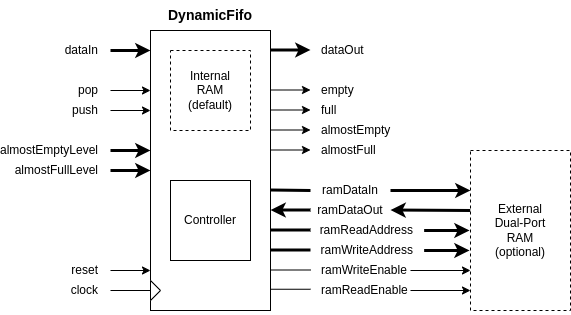
\includegraphics[width=0.80\textwidth]{images/block-diagram.png}
  \caption{Block Diagram}\label{fig:block-diagram}
\end{figure}

The Timer module provides the following outputs:

\begin{itemize}[noitemsep]
  \item{\textit{count}: Current value of the counter.}
  \item{\textit{maxReached}: Signal indicating the counter has reached its maximum value.}
  \item{\textit{pwm}: PWM output signal with a duty cycle controlled by \textit{pwmCeiling}.}
  \item{\textit{interrupt}: Interrupt signal indicating timer events (e.g., max reached).}
\end{itemize}

\subsection{Interface Timing}
The Timer operates on a synchronous clock and provides outputs that are valid on the rising edge of the clock. The timing diagram below illustrates the behavior of the Timer when the counter reaches its maximum value and generates an interrupt.

% \begin{figure}[h]
%   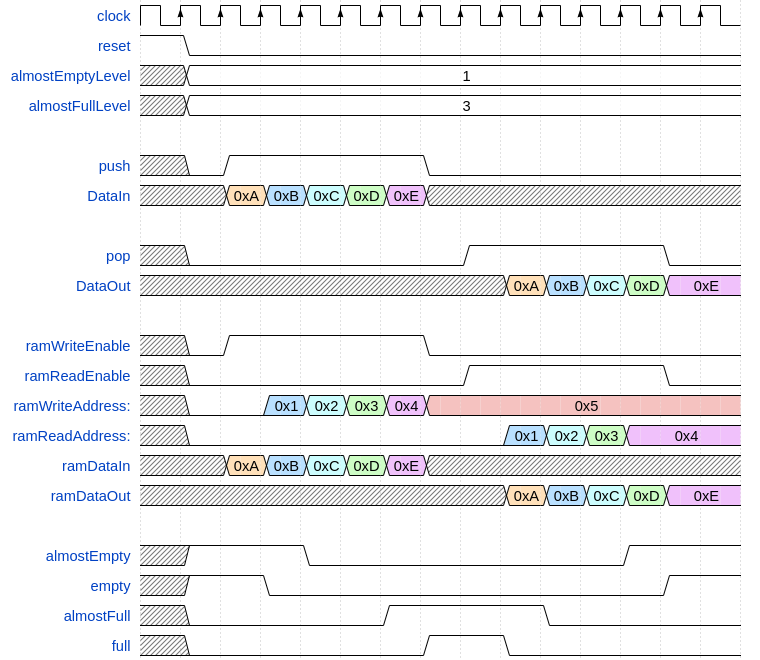
\includegraphics[width=\textwidth]{images/timing.png}
%   \caption{Timing Diagram}\label{fig:timing}
% \end{figure}
\section{Register Interface}

The UART module is controlled via an APB interface that maps configuration, status, and data registers for both the transmitter (TX) and receiver (RX) sections. In the updated design, the module uses internal dynamic FIFOs to buffer data and a dedicated baud–rate generator to compute the effective clocks–per–bit. This section describes the register map and details the functionality of each register.

\subsection{Register Map Summary}

The table below summarizes the complete register space. All addresses assume a 32–bit APB data bus. Note that some registers (e.g. TX\_CLOCKS\_PER\_BIT and RX\_CLOCKS\_PER\_BIT) are computed dynamically and are read–only.
It should be noted that all registers are \textbf{Double Buffered} and are automatically synchronized. This means that settings can be configured without the need for software synchronization.

\renewcommand*{\arraystretch}{1.25}
\begingroup
\small
\rowcolors{2}{gray!30}{gray!10}
\arrayrulecolor{gray!80}
\begin{longtable}{|c|c|c|c|p{0.35\textwidth}|}
    \hline
    \rowcolor{gray}
    \textcolor{white}{\textbf{Relative Address}} & \textcolor{white}{\textbf{Register Name}} & \textcolor{white}{\textbf{Type}} & \textcolor{white}{\textbf{Reset Value}} & \textcolor{white}{\textbf{Description}} \\ \hline
    \endfirsthead

    \hline
    \rowcolor{gray}
    \textcolor{white}{\textbf{Relative Address}} & \textcolor{white}{\textbf{Register Name}} & \textcolor{white}{\textbf{Type}} & \textcolor{white}{\textbf{Reset Value}} & \textcolor{white}{\textbf{Description}} \\ \hline
    \endhead

    \hline
    \endfoot

    0x0 &
    TX\_LOAD\_OFFSET &
    R/W &
    0 &
    When set to 1, all data in the TX fifo is sent out sequentially. It is automatically reset to 0 and does not have to be reset.
    \\ \hline

    0x4 &
    TX\_DATAIN\_OFFSET &
    R/W & 0 &
    When set, the data is sent to the back of the TX FIFO. It is automatically reset to 0 and does not have to be reset.
    \\ \hline

    0x8 &
    TX\_BAUDRATE\_OFFSET &
    R/W &
    115,200 &
    Controls the baud rate of the module. Is updated after TX\_UPDATEBAUD is asserted.
    \\ \hline

    0xC &
    TX\_CLOCKFREQ\_OFFSET &
    R/W &
    25,000,000 &
    This does not control the clock frequency, it is used by the divider to configure the TX frequency and must match the module clock frequency. Is updated after TX\_UPDATEBAUD is asserted.
    \\ \hline

    0x10 &
    TX\_UPDATEBAUD\_OFFSET &
    R/W &
    0 &
    This tells the TX module to apply the changes in TX\_BAUDRATE, and TX\_CLOCKFREQ. It can take up to 32 cycles to converge.
    \\ \hline

    0x14 &
    TX\_NUMOUTPUTBITSDB\_OFFSET &
    R/W &
    8 &
    This controls the number of data bits in a TX transaction.
    \\ \hline


    0x18 &
    TX\_USEPARITYDB\_OFFSET &
    R/W &
    0 &
    This controls whether to use a parity bit in a TX transaction.
    \\ \hline

    0x1C &
    TX\_PARITYODDDB\_OFFSET &
    R/W &
    0 &
    This controls whether to use odd or even parity in a TX transaction.
    \\ \hline

    0x20 &
    TX\_ALMOSTEMPTYLEVEL\_OFFSET &
    R/W &
    1 &
    This is the level of the TX FIFO that triggers the TX\_FIFOALMOSTEMPTY flag.
    \\ \hline

    0x24 &
    TX\_ALMOSTFULLLEVEL\_OFFSET &
    R/W &
    bufferSize - 1 &
    This is the level of the TX FIFO that triggers the TX\_FIFOALMOSTFULL flag.
    \\ \hline

    0x28 &
    TX\_FIFOFULL\_OFFSET &
    R &
    0 &
    This flag is set when the TX FIFO is full.
    \\ \hline

    0x2C &
    TX\_FIFOEMPTY\_OFFSET &
    R &
    0 &
    This flag is set when the TX FIFO is empty.
    \\ \hline

    0x30 &
    TX\_FIFOALMOSTEMPTY\_OFFSET &
    R &
    0 &
    This flag is set when the TX FIFO is at or below the TX\_ALMOSTEMPTYLEVEL.
    \\ \hline

    0x34 &
    TX\_FIFOALMOSTFULL\_OFFSET &
    R &
    0 &
    This flag is set when the TX FIFO is at or above the TX\_ALMOSTFULLLEVEL.
    \\ \hline

    0x38 &
    RX\_DATA\_OFFSET &
    R &
    0 &
    Desc
    \\ \hline

    0x3C &
    RX\_DATAPEEK\_OFFSET &
    R &
    0 &
    Desc
    \\ \hline

    0x40 &
    RX\_DATAAVAILABLE\_OFFSET &
    R/W &
    0 &
    Desc
    \\ \hline

    0x44 &
    ERROR\_OFFSET &
    R/W &
    0 &
    Desc
    \\ \hline

    0x48 &
    CLEARERROR\_OFFSET &
    R/W &
    0 &
    Desc
    \\ \hline

    0x4C &
    RX\_BAUDRATE\_OFFSET &
    R/W &
    0 &
    Desc
    \\ \hline

    0x50 &
    RX\_CLOCKFREQ\_OFFSET &
    R/W &
    0 &
    Desc
    \\ \hline

    0x54 &
    RX\_UPDATEBAUD\_OFFSET &
    R/W &
    0 &
    Desc
    \\ \hline

    0x58 &
    RX\_NUMOUTPUTBITSDB\_OFFSET &
    R/W &
    0 &
    Desc
    \\ \hline

    0x5C &
    RX\_USEPARITYDB\_OFFSET &
    R/W &
    0 &
    Desc
    \\ \hline

    0x60 &
    RX\_PARITYODDDB\_OFFSET &
    R/W &
    0 &
    Desc
    \\ \hline

    0x64 &
    RX\_ALMOSTEMPTYLEVEL\_OFFSET &
    R/W &
    0 &
    Desc
    \\ \hline

    0x68 &
    RX\_ALMOSTFULLLEVEL\_OFFSET &
    R/W &
    0 &
    Desc
    \\ \hline

    0x6C &
    RX\_FIFOFULL\_OFFSET &
    R/W &
    0 &
    Desc
    \\ \hline

    0x70 &
    RX\_FIFOEMPTY\_OFFSET &
    R/W &
    0 &
    Desc
    \\ \hline

    0x74 &
    RX\_FIFOALMOSTEMPTY\_OFFSET &
    R/W &
    0 &
    Desc
    \\ \hline

    0x78 &
    RX\_FIFOALMOSTFULL\_OFFSET &
    R/W &
    0 &
    Desc
    \\ \hline

    0x7C &
    RX\_CLOCKSPERBIT\_OFFSET &
    R/W &
    0 &
    Desc
    \\ \hline

    0x80 &
    TX\_CLOCKSPERBIT\_OFFSET &
    R/W &
    0 &
    Desc
    \\ \hline

    0x84 &
    RX\_LSBFIRST\_OFFSET &
    R/W &
    0 &
    Desc
    \\ \hline

    0x88 &
    TX\_LSBFIRST\_OFFSET &
    R/W &
    0 &
    Desc
    \\ \hline

    0x8C &
    RX\_FLUSH\_OFFSET &
    R/W &
    0 &
    Desc
    \\ \hline

    0x90 &
    TX\_FLUSH\_OFFSET &
    R/W &
    0 &
    Desc
    \\ \hline
\end{longtable}
\captionof{table}{UART Register Map}
\label{table:uart_register_map}
\endgroup

\subsection{Parameter Relationships and Calculations}

\textbf{Key Parameter Relationships:}
\begin{itemize}
    \item \texttt{dataWidth}: Width of the APB data bus (e.g., 32 bits).
    \item \texttt{maxOutputBits}: Maximum number of data bits per frame (excluding start/stop bits). An extra bit is provided for parity when enabled.
    \item \texttt{maxClockFrequency}: The maximum system clock frequency used by the baud generators (e.g., 25\,MHz).
    \item \texttt{maxBaudRate}: The highest supported baud rate (e.g., 921600 baud).
    \item \texttt{bufferSize}: Defines the depth of the internal dynamic FIFOs used in both TX and RX.
\end{itemize}

\textbf{Width Calculations:}
\begin{itemize}
    \item \texttt{TX\_DATA\_IN} / \texttt{RX\_DATA}: Width = \(\text{maxOutputBits}+1\). The extra bit is used to accommodate an optional parity bit.
    \item \texttt{TX\_NUM\_OUTPUT\_BITS\_DB} / \texttt{RX\_NUM\_OUTPUT\_BITS\_DB}: Width = \(\lceil\log_2(\text{maxOutputBits})\rceil+1\).

    \textit{Example:} For \(\text{maxOutputBits}=8\), the width is \(\lceil\log_2(8)\rceil+1 = 3+1 = 4\) bits.

    \item \texttt{TX\_CLOCKS\_PER\_BIT} / \texttt{RX\_CLOCKS\_PER\_BIT}: Width = \(\lceil\log_2(\tfrac{\text{maxClockFrequency}}{\text{maxBaudRate}})\rceil+1\).

    \textit{Example:} For a 25\,MHz clock and 921600 baud, the width is \(\lceil\log_2(25\,000\,000/921600)\rceil+1 \approx \lceil4.76\rceil+1 = 5+1 = 6\) bits.
\end{itemize}

\subsection{Key Register Descriptions}

\subsubsection{TX\_DATA\_IN (Address 0x00)}
\begin{itemize}[noitemsep]
    \item \textbf{Function:} Holds the data word to be transmitted.
    \item \textbf{Usage:} Software writes the desired value (e.g., an 8-bit word with an extra parity bit if used) before triggering transmission.
    \item \textbf{Reset Value:} 0x000.
\end{itemize}

\subsubsection{TX\_LOAD (Address 0x04)}
\begin{itemize}[noitemsep]
    \item \textbf{Function:} Triggers the transfer of the content in TX\_DATA\_IN into the TX FIFO.
    \item \textbf{Usage:} Write ‘1’ to this register to push the data into the FIFO. It auto–clears after one cycle.
    \item \textbf{Reset Value:} 0x0.
\end{itemize}

\subsubsection{TX\_BAUD\_RATE (Address 0x08) \& TX\_CLOCK\_FREQ (Address 0x0C)}
\begin{itemize}[noitemsep]
    \item \textbf{Function:}
    \begin{itemize}
        \item TX\_BAUD\_RATE sets the desired baud rate (e.g., 115200).
        \item TX\_CLOCK\_FREQ specifies the system clock frequency driving the baud generator.
    \end{itemize}
    \item \textbf{Usage:} After writing these registers, software must pulse TX\_UPDATE\_BAUD to update the baud divisor.
    \item \textbf{Reset Values:} 115200 and 25,000,000 respectively.
\end{itemize}

\subsubsection{TX\_UPDATE\_BAUD (Address 0x10)}
\begin{itemize}[noitemsep]
    \item \textbf{Function:} Triggers an update of the TX baud divisor.
    \item \textbf{Usage:} A pulse (write ‘1’) causes the UartBaudRateGenerator to compute a new \texttt{clocksPerBit} value, which is then stored in TX\_CLOCKS\_PER\_BIT.
    \item \textbf{Reset Value:} 0x0.
\end{itemize}

\subsubsection{TX\_NUM\_OUTPUT\_BITS\_DB (Address 0x14)}
\begin{itemize}[noitemsep]
    \item \textbf{Function:} Configures the number of data bits to be transmitted.
    \item \textbf{Usage:} Valid values typically range from 5 to \texttt{maxOutputBits}. The setting takes effect on the next transmission.
    \item \textbf{Reset Value:} 0x8 (for an 8-bit frame).
\end{itemize}

\subsubsection{TX\_USE\_PARITY\_DB (Address 0x18) and TX\_PARITY\_ODD\_DB (Address 0x1C)}
\begin{itemize}[noitemsep]
    \item \textbf{Function:}
    \begin{itemize}
        \item TX\_USE\_PARITY\_DB enables parity generation when set to ‘1’.
        \item TX\_PARITY\_ODD\_DB selects odd parity if ‘1’; if ‘0’, even parity is used.
    \end{itemize}
    \item \textbf{Usage:} Set these registers appropriately to control parity on transmission.
    \item \textbf{Reset Values:} Both default to 0 (parity disabled).
\end{itemize}

\subsubsection{TX\_CLOCKS\_PER\_BIT (Address 0x20)}
\begin{itemize}[noitemsep]
    \item \textbf{Function:} Contains the calculated number of clock cycles per transmitted bit.
    \item \textbf{Usage:} This read–only value is computed by the TX baud generator after a TX\_UPDATE\_BAUD pulse.
    \item \textbf{Reset Value:} Dynamically calculated.
\end{itemize}

\subsubsection{RX\_DATA (Address 0x24)}
\begin{itemize}[noitemsep]
    \item \textbf{Function:} Holds the data word received by the UART.
    \item \textbf{Usage:} After successful reception and FIFO push, software reads RX\_DATA to retrieve the word.
    \item \textbf{Reset Value:} 0x000.
\end{itemize}

\subsubsection{RX\_DATA\_AVAILABLE (Address 0x28)}
\begin{itemize}[noitemsep]
    \item \textbf{Function:} Indicates whether new data is available in the RX FIFO.
    \item \textbf{Usage:} Poll this register to determine when data is ready for reading.
    \item \textbf{Reset Value:} 0x0.
\end{itemize}

\subsubsection{RX\_ERROR (Address 0x2C)}
\begin{itemize}[noitemsep]
    \item \textbf{Function:} Reports reception errors:
    \begin{itemize}
        \item 00: No error.
        \item 01: Parity error.
        \item 10: Framing error.
        \item 11: Overrun error.
    \end{itemize}
    \item \textbf{Usage:} Monitor this register to detect errors; errors are cleared by writing to RX\_CLEAR\_ERROR.
    \item \textbf{Reset Value:} 0x0.
\end{itemize}

\subsubsection{TOP\_ERROR (Address 0x30)}
\begin{itemize}[noitemsep]
    \item \textbf{Function:} Indicates configuration or top–level errors.
    \item \textbf{Usage:} Software should check this register to ensure the module is correctly configured.
    \item \textbf{Reset Value:} 0x0.
\end{itemize}

\subsubsection{RX\_CLEAR\_ERROR (Address 0x34)}
\begin{itemize}[noitemsep]
    \item \textbf{Function:} Clears the RX error flags (in RX\_ERROR).
    \item \textbf{Usage:} Write ‘1’ to reset any error status.
    \item \textbf{Reset Value:} 0x0.
\end{itemize}

\subsubsection{RX\_BAUD\_RATE (Address 0x38) and RX\_CLOCK\_FREQ (Address 0x3C)}
\begin{itemize}[noitemsep]
    \item \textbf{Function:}
    \begin{itemize}
        \item RX\_BAUD\_RATE: Desired baud rate for reception.
        \item RX\_CLOCK\_FREQ: System clock frequency for the RX baud generator.
    \end{itemize}
    \item \textbf{Usage:} Configure these values similarly to the TX side.
    \item \textbf{Reset Values:} 115200 for RX\_BAUD\_RATE and 25,000,000 for RX\_CLOCK\_FREQ.
\end{itemize}

\subsubsection{RX\_UPDATE\_BAUD (Address 0x40)}
\begin{itemize}[noitemsep]
    \item \textbf{Function:} Triggers an update of the RX baud divisor.
    \item \textbf{Usage:} Pulse ‘1’ to have the UartBaudRateGenerator recalculate the effective clocks–per–bit.
    \item \textbf{Reset Value:} 0x0.
\end{itemize}

\subsubsection{RX\_NUM\_OUTPUT\_BITS\_DB (Address 0x44)}
\begin{itemize}[noitemsep]
    \item \textbf{Function:} Sets the expected number of data bits per received frame.
    \item \textbf{Usage:} This value must match the transmitter’s setting to avoid framing errors.
    \item \textbf{Reset Value:} 0x8.
\end{itemize}

\subsubsection{RX\_USE\_PARITY\_DB (Address 0x48) and RX\_PARITY\_ODD\_DB (Address 0x4C)}
\begin{itemize}[noitemsep]
    \item \textbf{Function:}
    \begin{itemize}
        \item RX\_USE\_PARITY\_DB: Enables parity checking when set to ‘1’.
        \item RX\_PARITY\_ODD\_DB: Selects odd parity if ‘1’ (even parity if ‘0’).
    \end{itemize}
    \item \textbf{Usage:} Configure these registers as needed for the desired parity configuration.
    \item \textbf{Reset Values:} Both default to 0.
\end{itemize}

\subsubsection{RX\_CLOCKS\_PER\_BIT (Address 0x50)}
\begin{itemize}[noitemsep]
    \item \textbf{Function:} Contains the computed number of system clock cycles per received bit.
    \item \textbf{Usage:} This read–only value is generated by the RX baud generator and used internally for sampling.
    \item \textbf{Reset Value:} Calculated dynamically.
\end{itemize}

\subsection{Programming Template}

Below is an example header file and source file to use the Uart module.

\subsubsection{Header File}

\begin{lstlisting}[language=C,frame=single,label={lst:header}]

#ifndef REGISTER_MAP_H
#define REGISTER_MAP_H

#define TX_LOAD_OFFSET 0x0
#define TX_DATAIN_OFFSET 0x4
#define TX_BAUDRATE_OFFSET 0x8
#define TX_CLOCKFREQ_OFFSET 0xC
#define TX_UPDATEBAUD_OFFSET 0x10
#define TX_NUMOUTPUTBITSDB_OFFSET 0x14
#define TX_USEPARITYDB_OFFSET 0x18
#define TX_PARITYODDDB_OFFSET 0x1C
#define TX_ALMOSTEMPTYLEVEL_OFFSET 0x20
#define TX_ALMOSTFULLLEVEL_OFFSET 0x24
#define TX_FIFOFULL_OFFSET 0x28
#define TX_FIFOEMPTY_OFFSET 0x2C
#define TX_FIFOALMOSTEMPTY_OFFSET 0x30
#define TX_FIFOALMOSTFULL_OFFSET 0x34
#define RX_DATA_OFFSET 0x38
#define RX_DATAPEEK_OFFSET 0x3C
#define RX_DATAAVAILABLE_OFFSET 0x40
#define ERROR_OFFSET 0x44
#define CLEARERROR_OFFSET 0x48
#define RX_BAUDRATE_OFFSET 0x4C
#define RX_CLOCKFREQ_OFFSET 0x50
#define RX_UPDATEBAUD_OFFSET 0x54
#define RX_NUMOUTPUTBITSDB_OFFSET 0x58
#define RX_USEPARITYDB_OFFSET 0x5C
#define RX_PARITYODDDB_OFFSET 0x60
#define RX_ALMOSTEMPTYLEVEL_OFFSET 0x64
#define RX_ALMOSTFULLLEVEL_OFFSET 0x68
#define RX_FIFOFULL_OFFSET 0x6C
#define RX_FIFOEMPTY_OFFSET 0x70
#define RX_FIFOALMOSTEMPTY_OFFSET 0x74
#define RX_FIFOALMOSTFULL_OFFSET 0x78
#define RX_CLOCKSPERBIT_OFFSET 0x7C
#define TX_CLOCKSPERBIT_OFFSET 0x80
#define RX_LSBFIRST_OFFSET 0x84
#define TX_LSBFIRST_OFFSET 0x88
#define RX_FLUSH_OFFSET 0x8C
#define TX_FLUSH_OFFSET 0x90

#endif REGISTER_MAP_H
\end{lstlisting}

\subsubsection{TX Source File}
\begin{lstlisting}[language=C,frame=single,label={lst:tx-source}]

#include <stdio.h>
#include <stdlib.h>
#include <fcntl.h>
#include <unistd.h>
#include <sys/mman.h>
#include <stdint.h>
#include "uartRegs.h"

// Base address for the UART registers and mapping size
#define UART_BASE 0x43C20000
#define REG_SIZE  0x1000

// Transmitter register offsets (32-bit registers)

// Hypothetical TX FIFO empty flag register offset.
// Assumed to return 1 when the FIFO is empty.
//#define TX_FIFO_EMPTY_OFFSET          0x60

int main(void)
{
    int fd = open("/dev/mem", O_RDWR | O_SYNC);
    if(fd < 0) {
        perror("Failed to open /dev/mem");
        return -1;
    }

    volatile uint8_t *base = mmap(NULL, REG_SIZE, PROT_READ | PROT_WRITE, MAP_SHARED, fd, UART_BASE);
    if(base == MAP_FAILED) {
        perror("Failed to mmap UART registers");
        close(fd);
        return -1;
    }

    // 1. Configure TX baud rate and data format
    *(volatile uint32_t *)(base + TX_CLOCKFREQ_OFFSET)         = 50000000;  // Set TX system clock frequency to 25 MHz
    *(volatile uint32_t *)(base + TX_BAUDRATE_OFFSET)            = 115200;    // Set desired baud rate to 115200
    *(volatile uint32_t *)(base + TX_UPDATEBAUD_OFFSET)          = 1;         // Trigger TX baud rate update
    *(volatile uint32_t *)(base + TX_NUMOUTPUTBITSDB_OFFSET)   = 8;         // Configure for 8 data bits per frame
    *(volatile uint32_t *)(base + TX_USEPARITYDB_OFFSET)        = 0;         // Disable parity
    *(volatile uint32_t *)(base + TX_PARITYODDDB_OFFSET)        = 0;         // (Ignored if parity is disabled)

    // 2. Enqueue data for transmission
    *(volatile uint32_t *)(base + TX_DATAIN_OFFSET) = 0x33;         // Write data word (0x55)
    *(volatile uint32_t *)(base + TX_LOAD_OFFSET)    = 1;            // Pulse 'load' to push data into TX FIFO

    printf("Data transmitted successfully.\n");

    munmap((void *)base, REG_SIZE);
    close(fd);
    return 0;
}
\end{lstlisting}

\subsubsection{RX Source File}
\begin{lstlisting}[language=C,frame=single,label={lst:rx-source}]
#include <stdio.h>
#include <stdlib.h>
#include <fcntl.h>
#include <unistd.h>
#include <sys/mman.h>
#include <stdint.h>
#include "uartRegs.h"

#define UART_BASE 0x43C30000
#define REG_SIZE  0x1000

// Receiver register offsets (32-bit registers)
// Hypothetical register to indicate that data has been read (pop the RX FIFO)
// Not in the original map but referenced by the pseudocode.

int main(void)
{
    int fd = open("/dev/mem", O_RDWR | O_SYNC);
    if(fd < 0) {
        perror("Failed to open /dev/mem");
        return -1;
    }

    volatile uint8_t *base = mmap(NULL, REG_SIZE, PROT_READ | PROT_WRITE, MAP_SHARED, fd, UART_BASE);
    if(base == MAP_FAILED) {
        perror("Failed to mmap UART registers");
        close(fd);
        return -1;
    }

    // 1. Configure RX baud rate and data format
    *(volatile uint32_t *)(base + RX_CLOCKFREQ_OFFSET)         = 50000000;  // Set RX system clock frequency to 25 MHz
    *(volatile uint32_t *)(base + RX_BAUDRATE_OFFSET)            = 115200;    // Set desired baud rate to 115200
    *(volatile uint32_t *)(base + RX_UPDATEBAUD_OFFSET)          = 1;         // Trigger RX baud rate update
    *(volatile uint32_t *)(base + RX_NUMOUTPUTBITSDB_OFFSET)   = 8;         // Configure for 8 data bits per frame
    *(volatile uint32_t *)(base + RX_USEPARITYDB_OFFSET)        = 0;         // Disable parity
    *(volatile uint32_t *)(base + RX_PARITYODDDB_OFFSET)        = 0;         // (Ignored if parity is disabled)

    // 2. Poll for data reception: wait until RX FIFO is not empty.
    // (Assuming RX_DATA_AVAILABLE returns a nonzero value when data is available.)
    while(*(volatile uint32_t *)(base + RX_DATAAVAILABLE_OFFSET) == 0) {
        usleep(1000);        // Wait for data to be received
    }

    // 3. Read the received data word
    uint32_t rx_data = *(volatile uint32_t *)(base + RX_DATA_OFFSET);
    printf("Received data: 0x%02X\n", rx_data);

    // 5. Check for any reception errors
    uint32_t err = *(volatile uint32_t *)(base + TOP_ERROR_OFFSET);
    if(err != 0) {
        printf("UART RX error: 0x%02X. Clearing error...\n", err);
        *(volatile uint32_t *)(base + CLEARERROR_OFFSET) = 1;
    }

    munmap((void *)base, REG_SIZE);
    close(fd);
    return 0;
}
\end{lstlisting}

\subsection{Configuration Workflow}

A typical configuration sequence is as follows:

\begin{enumerate}[noitemsep]
    \item \textbf{Set Baud Rates:}
    \begin{itemize}[noitemsep]
        \item Write the desired baud rate to TX\_BAUD\_RATE and RX\_BAUD\_RATE.
        \item Write the system clock frequency to TX\_CLOCK\_FREQ and RX\_CLOCK\_FREQ.
        \item Pulse TX\_UPDATE\_BAUD and RX\_UPDATE\_BAUD to trigger the baud generators.
    \end{itemize}

    \item \textbf{Configure Data Format:}
    \begin{itemize}[noitemsep]
        \item Set TX\_NUM\_OUTPUT\_BITS\_DB and RX\_NUM\_OUTPUT\_BITS\_DB to the desired number of data bits.
        \item Enable parity via TX\_USE\_PARITY\_DB and RX\_USE\_PARITY\_DB, and select odd/even with TX\_PARITY\_ODD\_DB and RX\_PARITY\_ODD\_DB if required.
    \end{itemize}

    \item \textbf{Initiate Transmission:}
    \begin{itemize}[noitemsep]
        \item Write the data word to TX\_DATA\_IN.
        \item Pulse TX\_LOAD to enqueue the data into the TX FIFO.
    \end{itemize}

    \item \textbf{Data Reception:}
    \begin{itemize}[noitemsep]
        \item Poll RX\_DATA\_AVAILABLE to determine if new data is ready.
        \item When available, issue a pop command (e.g., via a register control such as RX\_READ) and read RX\_DATA.
        \item Check RX\_ERROR for any reception errors and clear them using RX\_CLEAR\_ERROR.
    \end{itemize}
\end{enumerate}

\subsection{Error Conditions}

The UART module detects several error conditions:
\begin{itemize}[noitemsep]
    \item \textbf{Parity Error:} Occurs when parity checking is enabled and the received parity bit does not match the computed parity.
    \item \textbf{Framing Error:} Triggered when the expected stop bit is not detected.
    \item \textbf{Overrun Error:} Occurs if new data arrives before the previous word has been read from the RX FIFO.
    \item \textbf{Configuration Error:} Invalid configuration values (e.g., mismatched data bit settings) may trigger TOP\_ERROR.
\end{itemize}
Errors are reported in RX\_ERROR and can be cleared by writing ‘1’ to RX\_CLEAR\_ERROR.


\section{Simulation}

\subsection{Tests}
The test bench for the Timer module includes directed tests that verify the functionality of the counter, PWM generation, and interrupt signaling. The tests cover the following scenarios:

\begin{itemize}
  \item{Basic counter operation with and without a prescaler.}
  \item{PWM generation with varying duty cycles.}
  \item{Interrupt generation when the counter reaches its maximum value.}
\end{itemize}

\subsection{Code Coverage}
All inputs and outputs are checked to ensure they toggle at least once during simulation. An error will be thrown if any port fails to toggle.

\subsection{Running Simulation}
Simulations can be run directly from the command prompt as follows:

\begin{verbatim}
  $ sbt "test"
\end{verbatim}

or from make as follows:

\texttt{\$ make test}
\section{Synthesis}

\subsection{Area and Gate Count}
Example synthesis results vary based on \texttt{fifoDepth} and other settings. An illustrative table:

\renewcommand*{\arraystretch}{1.3}
\begingroup
\small
\rowcolors{2}{gray!30}{gray!10}
\begin{longtable}[H]{
  | p{0.22\textwidth}
  | p{0.18\textwidth}
  | p{0.20\textwidth}
  | p{0.30\textwidth} |
}
\hline
\rowcolor{gray}
\textcolor{white}{\textbf{Config}} &
\textcolor{white}{\textbf{FIFO Depth}} &
\textcolor{white}{\textbf{Data Bits}} &
\textcolor{white}{\textbf{Gate Count}} \\ 
\hline
\endfirsthead

\hline
\rowcolor{gray}
\textcolor{white}{\textbf{Config}} &
\textcolor{white}{\textbf{FIFO Depth}} &
\textcolor{white}{\textbf{Data Bits}} &
\textcolor{white}{\textbf{Gate Count}} \\ 
\hline
\endhead

\hline
\endfoot

\texttt{uart\_8\_depth4}  & 4  & 8  & 2,200 gates \\ \hline
\texttt{uart\_8\_depth16} & 16 & 8  & 3,100 gates \\ \hline
\texttt{uart\_9\_depth16} & 16 & 9  & 3,400 gates \\ \hline

\caption{Example Synthesis Results}
\end{longtable}
\endgroup

\subsection{Timing Constraints}
An \texttt{.sdc} file can be generated to specify clock period, input/output constraints, etc. For example:
\begin{verbatim}
create_clock -name PCLK -period 10.0 [get_ports PCLK]
set_input_delay 2.0 -clock PCLK [get_ports rx]
set_output_delay 2.0 -clock PCLK [get_ports tx]
\end{verbatim}

\subsection{Multicycle and False Paths}
Typically, no multicycle or false paths are required if the design runs entirely from \texttt{PCLK} with no asynchronous logic. Check your usage and tool warnings for final closure.

\section{Usage Examples}

This section demonstrates typical APB register write/read sequences for operating the UART module. The examples show how to configure the baud rate and data format, how to enqueue data for transmission via the TX FIFO, and how to read received data from the RX FIFO. These examples assume that the updated register interface uses a configuration bundle (e.g. \texttt{txConfig} for TX and \texttt{rxConfig} for RX) and that status signals (such as FIFO empty flags) are available for polling.

\subsection{Basic Transmit}

The following example shows how to configure the TX path, enqueue data into the TX FIFO, and wait for the transmission to complete.

\begin{verbatim}
// 1. Configure TX baud rate and data format
write(txConfig.clockFreq, 25000000);  // Set TX system clock frequency to 25 MHz
write(txConfig.baud, 115200);           // Set desired baud rate to 115200
write(txConfig.updateBaud, 1);          // Trigger TX baud rate update

write(txConfig.numOutputBitsDb, 8);     // Configure for 8 data bits per frame
write(txConfig.useParityDb, 0);         // Disable parity
write(txConfig.parityOddDb, 0);         // (Ignored if parity is disabled)

// 2. Enqueue data for transmission
write(txConfig.data, 0x55);             // Write data word (e.g., 0x55)
write(txConfig.load, 1);                // Pulse 'load' to push data into the TX FIFO

// 3. Wait until the TX FIFO is empty
while (read(txFifoEmpty) == 0) {
    // Poll status or yield until TX FIFO becomes empty
}
\end{verbatim}

\vspace{1em}
\noindent
\textbf{Explanation:}  
The transmitter configuration sets the baud rate using \texttt{txConfig.clockFreq} and \texttt{txConfig.baud} and then pulses \texttt{txConfig.updateBaud} to update the internal divisor. The data word is then loaded into \texttt{txConfig.data} and a pulse on \texttt{txConfig.load} pushes it into the internal dynamic FIFO. The transmitter automatically pops data from the FIFO and transmits it (LSB first, after an internal reversal) through the TX state machine.

\subsection{Basic Receive}

The following example demonstrates how to configure the RX path, poll for incoming data, read the received word from the FIFO, and clear any errors.

\begin{verbatim}
// 1. Configure RX baud rate and data format
write(rxConfig.clockFreq, 25000000);  // Set RX system clock frequency to 25 MHz
write(rxConfig.baud, 115200);           // Set desired baud rate to 115200
write(rxConfig.updateBaud, 1);          // Trigger RX baud rate update

write(rxConfig.numOutputBitsDb, 8);     // Configure for 8 data bits per frame
write(rxConfig.useParityDb, 0);         // Disable parity (set to 1 to enable)
write(rxConfig.parityOddDb, 0);         // (Ignored if parity is disabled)

// 2. Poll for data reception
while (read(rxFifoEmpty) == 1) {
    // Wait until RX FIFO is not empty (data available)
}

// 3. Read the received data word
uint32_t rx_data = read(rxData);

// 4. Indicate that the data has been read (pop from FIFO)
write(rxConfig.rxDataRegRead, 1);

// 5. Check for any reception errors
uint32_t err = read(rxError);
if (err != 0) {
    // Handle error (e.g., parity or framing error)
    // Clear errors by writing '1' to rxConfig.clearErrorDb
    write(rxConfig.clearErrorDb, 1);
}
\end{verbatim}

\vspace{1em}
\noindent
\textbf{Explanation:}  
The RX configuration is similar to TX. After setting the baud parameters and updating the divisor, the receiver continuously samples the asynchronous RX line. When a complete frame is received without error, it is pushed into the RX FIFO. Software polls the FIFO status (e.g., via \texttt{rxFifoEmpty}) until data is available, then reads the word from \texttt{rxData} and signals the FIFO to pop that data using \texttt{rxConfig.rxDataRegRead}. If errors are detected, the RX error register will indicate the type of error, and software can clear these by writing to \texttt{rxConfig.clearErrorDb}.

\subsection{Handling Parity}

The following example shows how to enable parity checking (odd parity in this case) and transmit data with parity enabled. On the RX side, parity is automatically checked against the expected odd parity.

\begin{verbatim}
// Enable odd parity on both TX and RX
write(txConfig.useParityDb, 1);
write(txConfig.parityOddDb, 1);

write(rxConfig.useParityDb, 1);
write(rxConfig.parityOddDb, 1);

// Transmit a byte with odd parity enabled
write(txConfig.data, 0xAB);  // Load data 0xAB into TX_DATA
write(txConfig.load, 1);       // Pulse 'load' to push the data into the TX FIFO

// The transmitter computes the parity bit from the full data word.
// On the RX side, if the parity bit does not match the computed value,
// the error register (rxError) will be updated with a ParityError.
\end{verbatim}

\vspace{1em}
\noindent
\textbf{Explanation:}  
By setting \texttt{useParityDb} to 1 and choosing odd parity with \texttt{parityOddDb}, the transmitter includes a computed parity bit after sending the data bits. The receiver, with the same settings, checks the incoming parity. A mismatch triggers a parity error, which software can detect by reading the \texttt{rxError} register.

---

These examples illustrate the step-by-step configuration and operation of the UART module using the updated register interface, including dynamic FIFO buffering and baud–rate updating. Adjust the register names and values to match your design specifics as needed.


\end{document}